\subsection{VGA driver}

VGA driver is the most complex peripheral of MARK II. It is display driver with
VGA output, working in text mode. Its parameters are:

\begin{itemize}
    \item Pixel clock: 31.5MHz
    \item Resolution: 640x480 @ 73Hz
    \item Text resolution: 80x30 chars
    \item Char resolution: 16x8 pixels
    \item Colors: 16 collors
    \item Charset: 128 ASCII chars with some pseudo graphics
\end{itemize}

\subsubsection{Function}

Although VGA driver is complex peripheral, it's controlling is really simple.
By the programmer, VGA driver is seen as simple memory. You can read from this
memory and you can also write to this memory. But this memory is only 15 bits
wide.

VGA driver is able to display only characters. It has it own char set that is
mostly compatible with ASCII codes. Char set is shown on figure
\ref{fig:MARK_II_charset}.

Except standard ASCII characters there are also some chars that can be used to
print pseudo graphics.

VGA driver also support colors. You can specify color for foreground (character
itself) and for background. There is sixteen kinds of colors. And are listed,
together with their codes in table \ref{tab:vga_colors_codes}.

\begin{figure}[h]
    \centering
    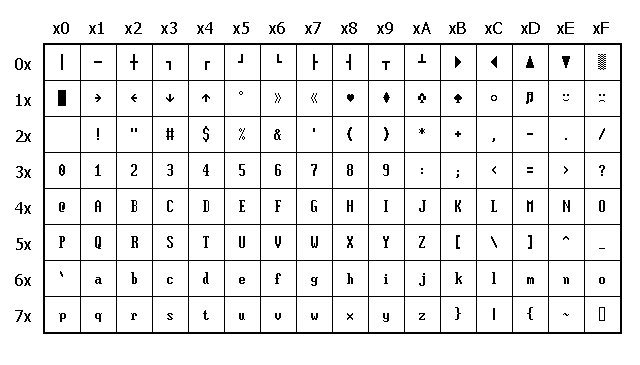
\includegraphics[width=.85\textwidth]{img/MARKII_charset.png}
    \caption{VGA driver character set}
    \label{fig:MARK_II_charset}
\end{figure}

\begin{table}[h]
    \centering
    \begin{tabular}{|l|l|}
        \hline
        \textbf{Color} & \textbf{Code}  \\ \hline
        $0000_{2}$     & black          \\ \hline
        $0001_{2}$     & light gray     \\ \hline
        $0010_{2}$     & red            \\ \hline
        $0011_{2}$     & light red      \\ \hline
        $0100_{2}$     & green          \\ \hline
        $0101_{2}$     & light green    \\ \hline
        $0110_{2}$     & brown          \\ \hline
        $0111_{2}$     & yellow         \\ \hline
        $1000_{2}$     & blue           \\ \hline
        $1001_{2}$     & light blue     \\ \hline
        $1010_{2}$     & magenta        \\ \hline
        $1011_{2}$     & light magenta  \\ \hline
        $1100_{2}$     & cyan           \\ \hline
        $1101_{2}$     & light cyan     \\ \hline
        $1110_{2}$     & gray           \\ \hline
        $1111_{2}$     & white          \\ \hline
    \end{tabular}
    \caption{VGA driver supported colors}
    \label{tab:vga_collors_codes}
\end{table}

Writing on VGA display can be done by writing char code to the specified memory
location. Coordinates where character appear on the display is given by memory
address where character is wrote.

Display is organized as two dimensional array of characters. Its sizes are 80
columns and 30 lines of characters.

This organization is in video ram too. Address of character in memory is given
by following expression:

$$
    Address = r * 80_{16} + c
$$

Where $r$ mean row and $c$ mean column. For example, we want write character to
sixth row and eight column. Address to write is:

$$
    Address = r * 80_{16} + c = 6 * 80_{16} + 8 = 308_{16}
$$

Remember, top left corner have coordinates $[0, 0]$.

One memory location have 15 bits, in these 15 bits are coded color for background,
color for foreground, and character to display in following fashion:

\begin{itemize}
    \item \textbf{Bits 6 down to 0} - Character code from figure \ref{fig:MARK_II_charset}.
    \item \textbf{Bits 10 down to 7} - Foreground color code.
    \item \textbf{Bits 14 down to 11} - Background color code.
\end{itemize}

\subsubsection{Hacking}

You can simply add second VGA driver to drive two monitors at same time. This
can be done simply by adding second instance of vga component.

\begin{lstlisting}[language=VHDL, frame=single]
entity vga is
    generic(
        BASE_ADDRESS: unsigned(23 downto 0) := x"000000"
    );
    port(
        clk_bus: in std_logic;
        address: in unsigned(23 downto 0);
        data_mosi: in unsigned(31 downto 0);
        data_miso: out unsigned(31 downto 0);
        WR: in std_logic;
        RD: in std_logic;
        ack: out std_logic;
        clk_31M5: in std_logic;
        h_sync: out std_logic;
        v_sync: out std_logic;
        red: out std_logic_vector(1 downto 0);
        green: out std_logic_vector(1 downto 0);
        blue: out std_logic_vector(1 downto 0)
    );
end entity vga;
\end{lstlisting}

Entity vga have standard bus interface for connecting to the system bus, plus
some extra special signals. These special signals are output to the VGA connector,
and clock input for pixel generator. Part of VGA driver is running at another
clock domain. This domain have to be clocked at $31,5MHz$. Input named clk\_bus
is standard system clock.

Signals h\_sync and v\_sync are horizontal and vertical synchronizations. Signals
red, green and blue are color signals and they should be connected to the DA converters.
